%\section{Empirical Performance}
\label{sec:experiments}
% Experimental results

% Graphs
\begin{figure}[h]
\centering
\subfigure[$P_2$-Distributed Options]{
\includegraphics[height=2in]{figures/rooms-options}
\label{fig:rooms-options}
}
\subfigure[Cumulative Return]{
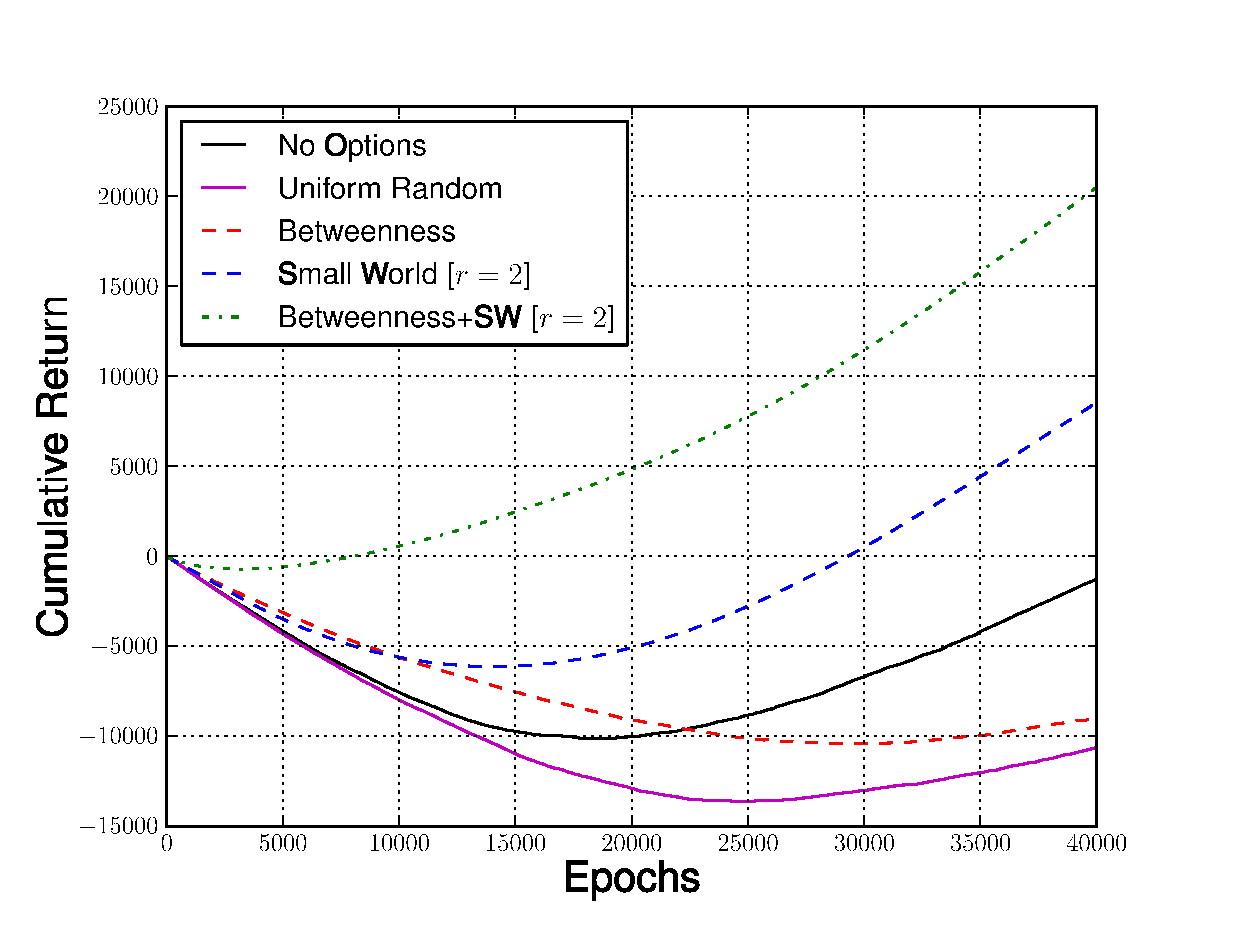
\includegraphics[height=2.2in]{figures/rooms-algos-200}
\label{fig:rooms-performance}
}
\label{fig:rooms}
\caption{Results on the Rooms Domain}
\end{figure}

% Brief description of Rooms, Taxi and Arbitrary Navigation domains.
We trained agents using the MacroQ algorithm, and tested it on three
standard domains, Taxi, Rooms and a $20\times20$ arbitrary navigation
task, and compared the performance of agents using options generated
(i) using betweenness centrality, (ii) using $P_0$ (uniformly random
paths), (iii) using paths between nodes selected using $P_{r>0}$, and
(iv) using a combination of (i) and (iii).  The performance of
$P_r$-distributed options was worst when $r=0$, and increased to peak
at a particular $r$ before decreasing again; behaviour also observed
in Kleinberg's work. With appropriate $r$, $P_r$-distributed options
accumulate significant return, and outperform bottleneck-based methods
on navigation tasks. 

% Observations
% When goal state and start state are further apart, the options that stand out
% are more

